% HPC campaign workflow (worker-pool + dependent job chain + resume gate).
% Standalone TikZ figure: `pdflatex hpc_workflow.tex` -> a tightly-cropped PDF,
% or % HPC campaign workflow (worker-pool + dependent job chain + resume gate).
% Standalone TikZ figure: `pdflatex hpc_workflow.tex` -> a tightly-cropped PDF,
% or % HPC campaign workflow (worker-pool + dependent job chain + resume gate).
% Standalone TikZ figure: `pdflatex hpc_workflow.tex` -> a tightly-cropped PDF,
% or % HPC campaign workflow (worker-pool + dependent job chain + resume gate).
% Standalone TikZ figure: `pdflatex hpc_workflow.tex` -> a tightly-cropped PDF,
% or \input{hpc_workflow} inside another document.
\documentclass[border=10pt]{standalone}
\usepackage{amsmath}
\usepackage{tikz}
\usetikzlibrary{arrows.meta, positioning, shapes.geometric, fit, backgrounds, calc}
\usepackage{xcolor}

\newcommand{\code}[1]{\texttt{\footnotesize\detokenize{#1}}}

\definecolor{cLogin}{HTML}{4683DE}
\definecolor{cJob}{HTML}{4BC55A}
\definecolor{cGate}{HTML}{FBA11B}
\definecolor{cBuild}{HTML}{966EBB}

\begin{document}
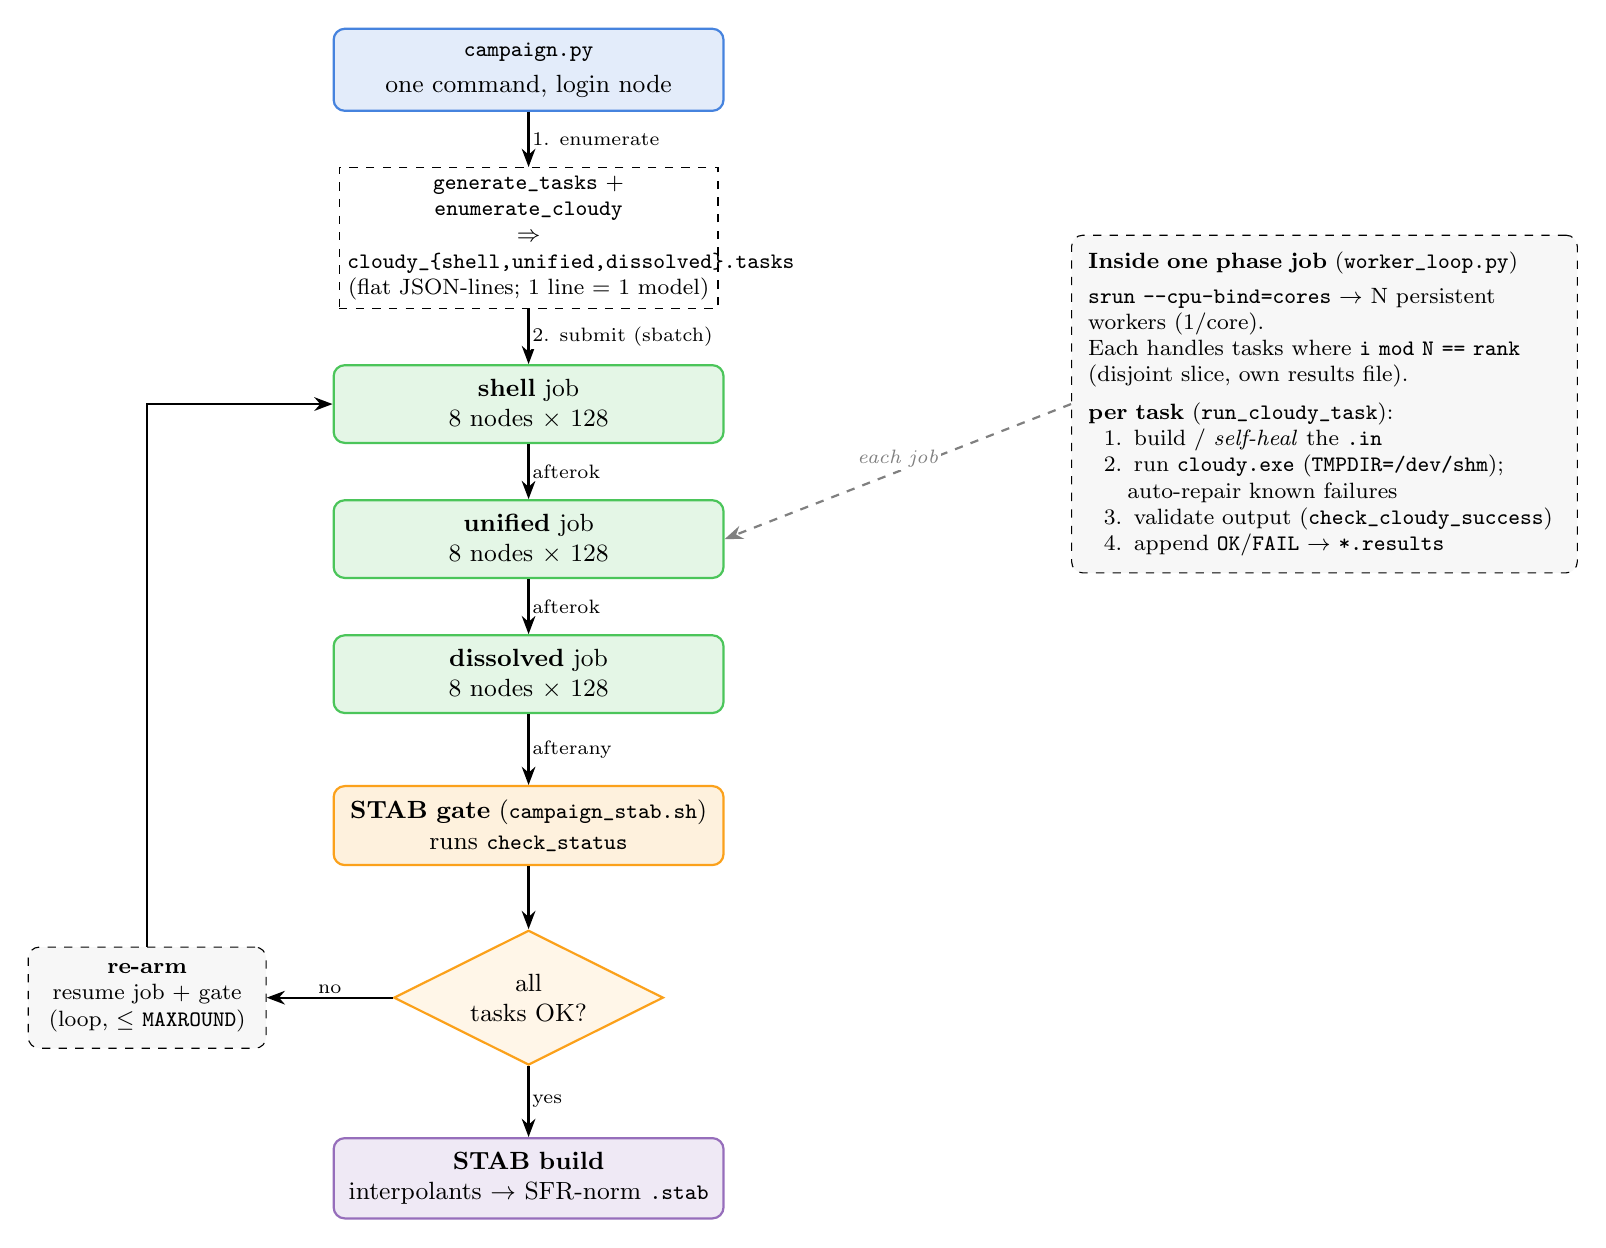
\begin{tikzpicture}[
  font=\small,
  >=Stealth,
  node distance = 7mm,
  pbox/.style   = {rectangle, rounded corners, draw, thick, align=center,
                   inner sep=5pt, text width=46mm},
  job/.style    = {pbox, fill=cJob!15, draw=cJob},
  login/.style  = {pbox, fill=cLogin!15, draw=cLogin},
  gate/.style   = {pbox, fill=cGate!15, draw=cGate},
  build/.style  = {pbox, fill=cBuild!15, draw=cBuild},
  dec/.style    = {diamond, aspect=2, draw, thick, align=center, inner sep=1pt,
                   fill=cGate!10, draw=cGate, text width=20mm},
  data/.style   = {rectangle, draw, dashed, align=center, font=\footnotesize,
                   inner sep=3pt, text width=46mm},
  detail/.style = {rectangle, rounded corners, draw, dashed, align=left,
                   font=\footnotesize, inner sep=6pt, text width=60mm, fill=black!3},
  arr/.style    = {->, thick},
  lab/.style    = {font=\scriptsize, fill=white, inner sep=1pt}]

% ---- left column: the orchestration chain ---------------------------------
\node[login] (camp) {\textbf{\code{campaign.py}}\\[2pt] one command, login node};
\node[data, below=of camp] (tasks)
   {\code{generate_tasks} + \code{enumerate_cloudy}\\
    $\Rightarrow$ \code{cloudy_{shell,unified,dissolved}.tasks}\\
    (flat JSON-lines; 1 line = 1 model)};
\node[job, below=of tasks] (shell)   {\textbf{shell} job\\ 8 nodes $\times$ 128};
\node[job, below=of shell] (unified) {\textbf{unified} job\\ 8 nodes $\times$ 128};
\node[job, below=of unified] (diss)  {\textbf{dissolved} job\\ 8 nodes $\times$ 128};
\node[gate, below=9mm of diss] (gate)
   {\textbf{STAB gate} (\code{campaign_stab.sh})\\ runs \code{check_status}};
\node[dec, below=8mm of gate] (dec) {all\\ tasks OK?};
\node[build, below=9mm of dec] (build)
   {\textbf{STAB build}\\ interpolants $\to$ SFR-norm \code{.stab}};

% chain arrows
\draw[arr] (camp) -- (tasks) node[lab, midway, right] {1. enumerate};
\draw[arr] (tasks) -- (shell) node[lab, midway, right] {2. submit (sbatch)};
\draw[arr] (shell) -- (unified) node[lab, midway, right] {afterok};
\draw[arr] (unified) -- (diss) node[lab, midway, right] {afterok};
\draw[arr] (diss) -- (gate) node[lab, midway, right] {afterany};
\draw[arr] (gate) -- (dec);
\draw[arr] (dec) -- node[lab, right] {yes} (build);

% ---- resume loop (no -> re-arm a fresh job + the gate, back to the top) ----
\node[detail, left=16mm of dec, text width=26mm, align=center] (resume)
  {\textbf{re-arm}\\ resume job + gate\\ (loop, $\le$ \code{MAXROUND})};
\draw[arr] (dec) -- node[lab, above] {no} (resume);
\draw[arr] (resume) |- (shell.west);

% ---- right: what one phase job actually does ------------------------------
\node[detail, right=44mm of shell, anchor=west] (worker)
  {\textbf{Inside one phase job} (\code{worker_loop.py})\\[3pt]
   \code{srun --cpu-bind=cores} $\to$ N persistent workers (1/core).\\
   Each handles tasks where \code{i mod N == rank} (disjoint
   slice, own results file).\\[4pt]
   \textbf{per task} (\code{run_cloudy_task}):\\
   \ \ 1. build / \emph{self-heal} the \code{.in}\\
   \ \ 2. run \code{cloudy.exe} (\code{TMPDIR=/dev/shm});\\
   \ \ \ \ \ auto-repair known failures\\
   \ \ 3. validate output (\code{check_cloudy_success})\\
   \ \ 4. append \code{OK}/\code{FAIL} $\to$ \code{*.results}};
\draw[arr, dashed, gray] (worker.west) -- (unified.east)
      node[lab, midway, above, font=\scriptsize\itshape] {each job};

% parallelism note (kept clear of the worker box, under the chain arrows)
\node[font=\scriptsize\itshape, align=center, below=1mm of diss, yshift=-0.5mm] {};

\end{tikzpicture}
\end{document}
 inside another document.
\documentclass[border=10pt]{standalone}
\usepackage{amsmath}
\usepackage{tikz}
\usetikzlibrary{arrows.meta, positioning, shapes.geometric, fit, backgrounds, calc}
\usepackage{xcolor}

\newcommand{\code}[1]{\texttt{\footnotesize\detokenize{#1}}}

\definecolor{cLogin}{HTML}{4683DE}
\definecolor{cJob}{HTML}{4BC55A}
\definecolor{cGate}{HTML}{FBA11B}
\definecolor{cBuild}{HTML}{966EBB}

\begin{document}
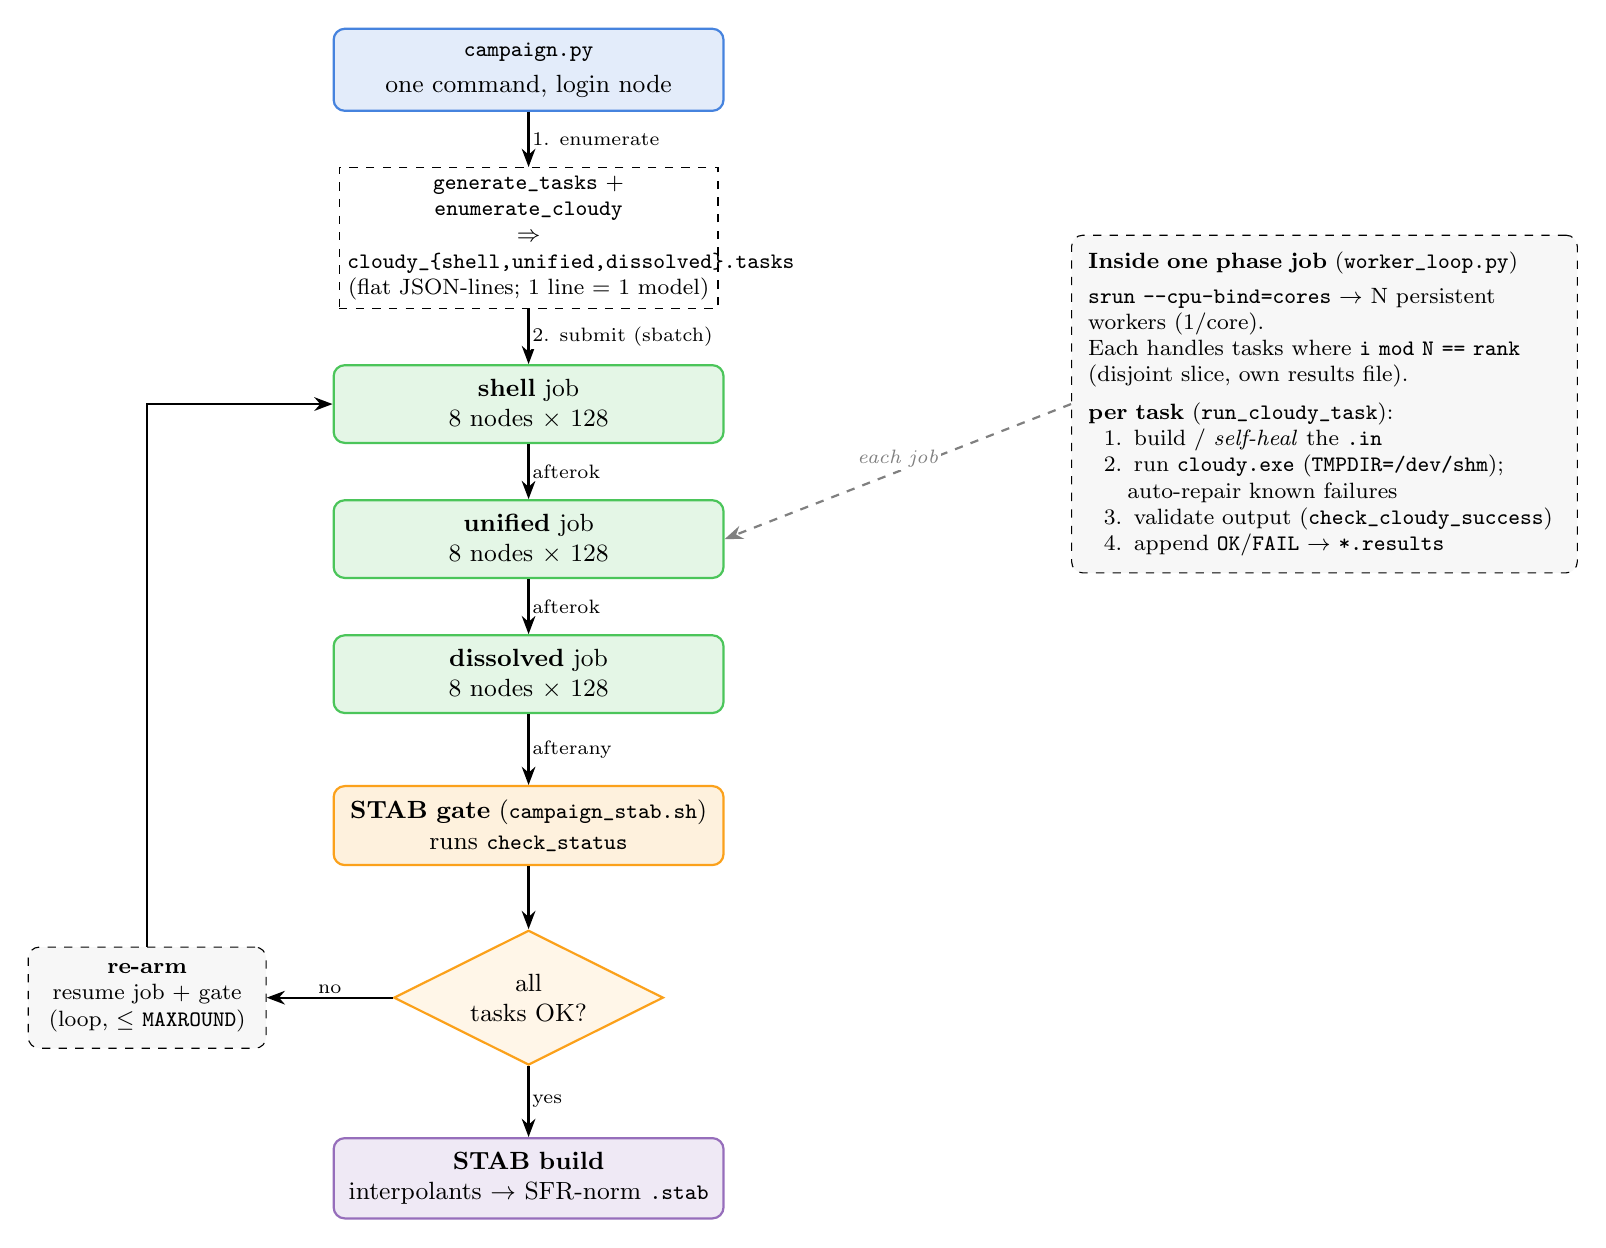
\begin{tikzpicture}[
  font=\small,
  >=Stealth,
  node distance = 7mm,
  pbox/.style   = {rectangle, rounded corners, draw, thick, align=center,
                   inner sep=5pt, text width=46mm},
  job/.style    = {pbox, fill=cJob!15, draw=cJob},
  login/.style  = {pbox, fill=cLogin!15, draw=cLogin},
  gate/.style   = {pbox, fill=cGate!15, draw=cGate},
  build/.style  = {pbox, fill=cBuild!15, draw=cBuild},
  dec/.style    = {diamond, aspect=2, draw, thick, align=center, inner sep=1pt,
                   fill=cGate!10, draw=cGate, text width=20mm},
  data/.style   = {rectangle, draw, dashed, align=center, font=\footnotesize,
                   inner sep=3pt, text width=46mm},
  detail/.style = {rectangle, rounded corners, draw, dashed, align=left,
                   font=\footnotesize, inner sep=6pt, text width=60mm, fill=black!3},
  arr/.style    = {->, thick},
  lab/.style    = {font=\scriptsize, fill=white, inner sep=1pt}]

% ---- left column: the orchestration chain ---------------------------------
\node[login] (camp) {\textbf{\code{campaign.py}}\\[2pt] one command, login node};
\node[data, below=of camp] (tasks)
   {\code{generate_tasks} + \code{enumerate_cloudy}\\
    $\Rightarrow$ \code{cloudy_{shell,unified,dissolved}.tasks}\\
    (flat JSON-lines; 1 line = 1 model)};
\node[job, below=of tasks] (shell)   {\textbf{shell} job\\ 8 nodes $\times$ 128};
\node[job, below=of shell] (unified) {\textbf{unified} job\\ 8 nodes $\times$ 128};
\node[job, below=of unified] (diss)  {\textbf{dissolved} job\\ 8 nodes $\times$ 128};
\node[gate, below=9mm of diss] (gate)
   {\textbf{STAB gate} (\code{campaign_stab.sh})\\ runs \code{check_status}};
\node[dec, below=8mm of gate] (dec) {all\\ tasks OK?};
\node[build, below=9mm of dec] (build)
   {\textbf{STAB build}\\ interpolants $\to$ SFR-norm \code{.stab}};

% chain arrows
\draw[arr] (camp) -- (tasks) node[lab, midway, right] {1. enumerate};
\draw[arr] (tasks) -- (shell) node[lab, midway, right] {2. submit (sbatch)};
\draw[arr] (shell) -- (unified) node[lab, midway, right] {afterok};
\draw[arr] (unified) -- (diss) node[lab, midway, right] {afterok};
\draw[arr] (diss) -- (gate) node[lab, midway, right] {afterany};
\draw[arr] (gate) -- (dec);
\draw[arr] (dec) -- node[lab, right] {yes} (build);

% ---- resume loop (no -> re-arm a fresh job + the gate, back to the top) ----
\node[detail, left=16mm of dec, text width=26mm, align=center] (resume)
  {\textbf{re-arm}\\ resume job + gate\\ (loop, $\le$ \code{MAXROUND})};
\draw[arr] (dec) -- node[lab, above] {no} (resume);
\draw[arr] (resume) |- (shell.west);

% ---- right: what one phase job actually does ------------------------------
\node[detail, right=44mm of shell, anchor=west] (worker)
  {\textbf{Inside one phase job} (\code{worker_loop.py})\\[3pt]
   \code{srun --cpu-bind=cores} $\to$ N persistent workers (1/core).\\
   Each handles tasks where \code{i mod N == rank} (disjoint
   slice, own results file).\\[4pt]
   \textbf{per task} (\code{run_cloudy_task}):\\
   \ \ 1. build / \emph{self-heal} the \code{.in}\\
   \ \ 2. run \code{cloudy.exe} (\code{TMPDIR=/dev/shm});\\
   \ \ \ \ \ auto-repair known failures\\
   \ \ 3. validate output (\code{check_cloudy_success})\\
   \ \ 4. append \code{OK}/\code{FAIL} $\to$ \code{*.results}};
\draw[arr, dashed, gray] (worker.west) -- (unified.east)
      node[lab, midway, above, font=\scriptsize\itshape] {each job};

% parallelism note (kept clear of the worker box, under the chain arrows)
\node[font=\scriptsize\itshape, align=center, below=1mm of diss, yshift=-0.5mm] {};

\end{tikzpicture}
\end{document}
 inside another document.
\documentclass[border=10pt]{standalone}
\usepackage{amsmath}
\usepackage{tikz}
\usetikzlibrary{arrows.meta, positioning, shapes.geometric, fit, backgrounds, calc}
\usepackage{xcolor}

\newcommand{\code}[1]{\texttt{\footnotesize\detokenize{#1}}}

\definecolor{cLogin}{HTML}{4683DE}
\definecolor{cJob}{HTML}{4BC55A}
\definecolor{cGate}{HTML}{FBA11B}
\definecolor{cBuild}{HTML}{966EBB}

\begin{document}
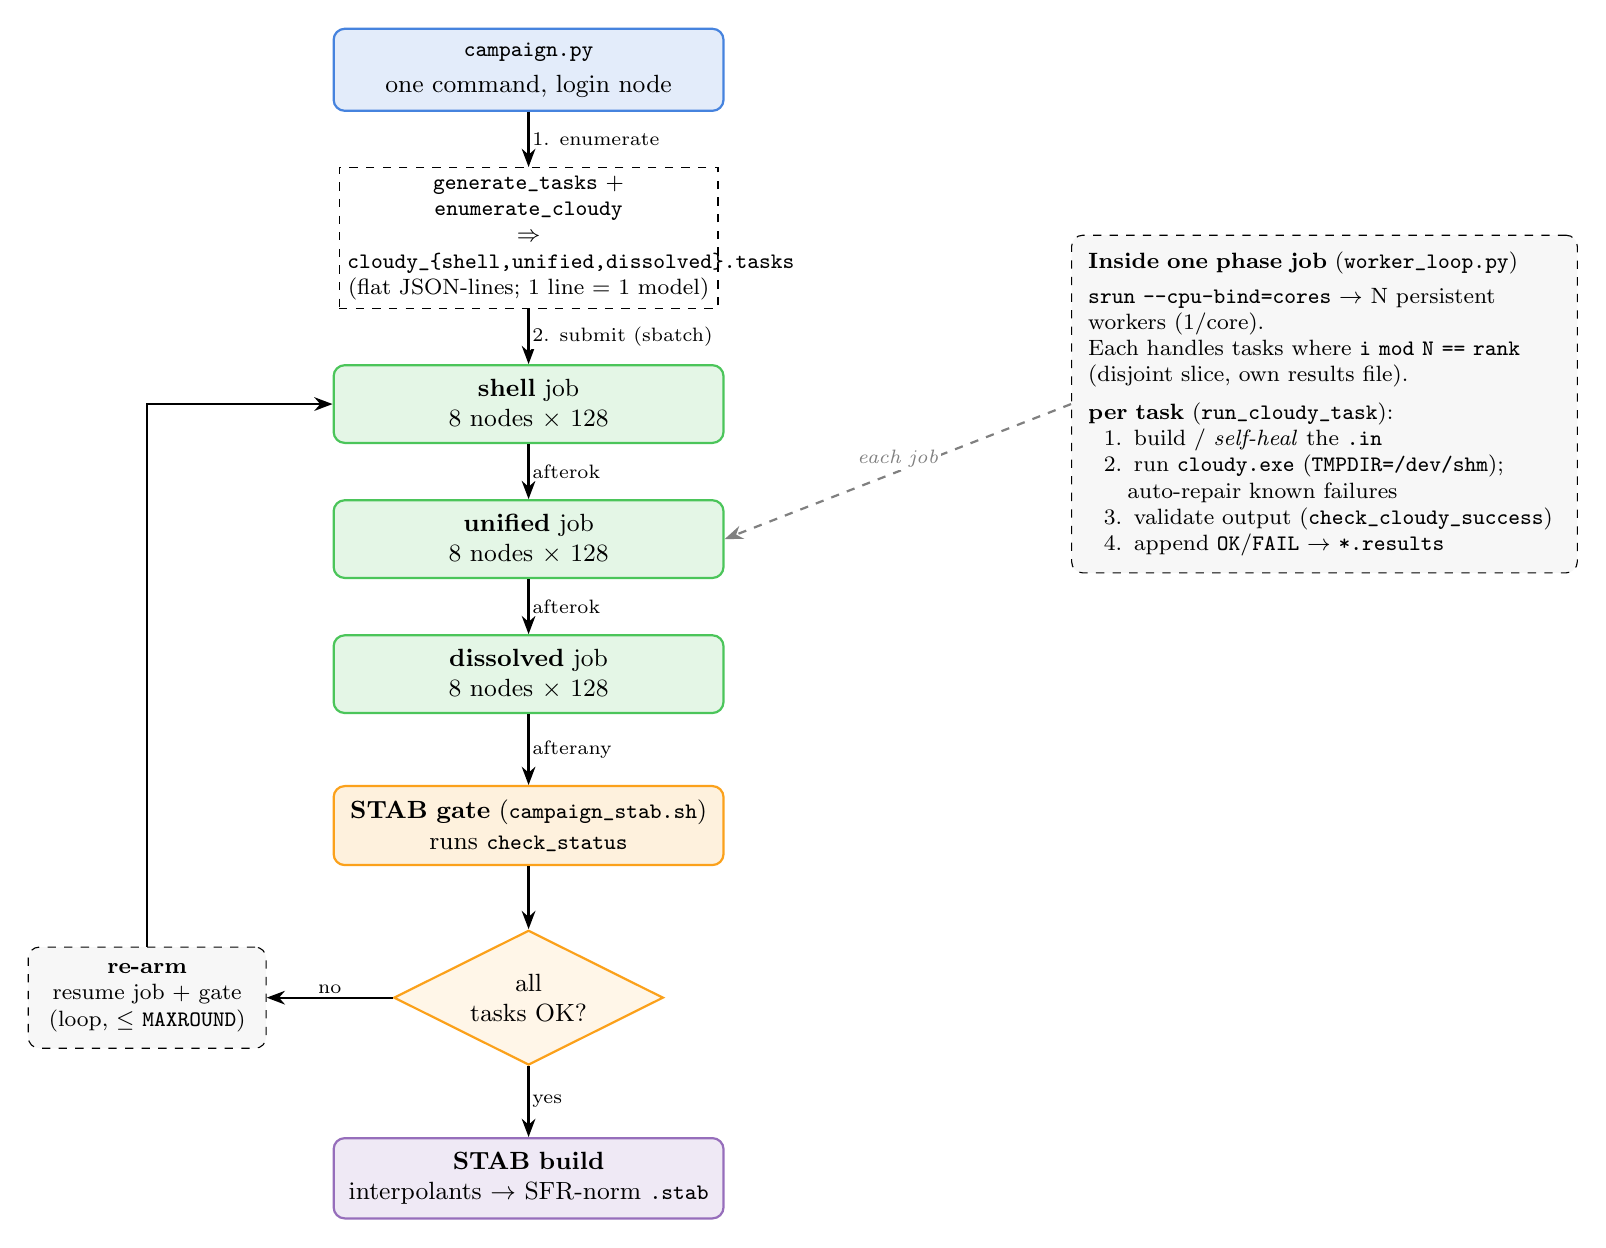
\begin{tikzpicture}[
  font=\small,
  >=Stealth,
  node distance = 7mm,
  pbox/.style   = {rectangle, rounded corners, draw, thick, align=center,
                   inner sep=5pt, text width=46mm},
  job/.style    = {pbox, fill=cJob!15, draw=cJob},
  login/.style  = {pbox, fill=cLogin!15, draw=cLogin},
  gate/.style   = {pbox, fill=cGate!15, draw=cGate},
  build/.style  = {pbox, fill=cBuild!15, draw=cBuild},
  dec/.style    = {diamond, aspect=2, draw, thick, align=center, inner sep=1pt,
                   fill=cGate!10, draw=cGate, text width=20mm},
  data/.style   = {rectangle, draw, dashed, align=center, font=\footnotesize,
                   inner sep=3pt, text width=46mm},
  detail/.style = {rectangle, rounded corners, draw, dashed, align=left,
                   font=\footnotesize, inner sep=6pt, text width=60mm, fill=black!3},
  arr/.style    = {->, thick},
  lab/.style    = {font=\scriptsize, fill=white, inner sep=1pt}]

% ---- left column: the orchestration chain ---------------------------------
\node[login] (camp) {\textbf{\code{campaign.py}}\\[2pt] one command, login node};
\node[data, below=of camp] (tasks)
   {\code{generate_tasks} + \code{enumerate_cloudy}\\
    $\Rightarrow$ \code{cloudy_{shell,unified,dissolved}.tasks}\\
    (flat JSON-lines; 1 line = 1 model)};
\node[job, below=of tasks] (shell)   {\textbf{shell} job\\ 8 nodes $\times$ 128};
\node[job, below=of shell] (unified) {\textbf{unified} job\\ 8 nodes $\times$ 128};
\node[job, below=of unified] (diss)  {\textbf{dissolved} job\\ 8 nodes $\times$ 128};
\node[gate, below=9mm of diss] (gate)
   {\textbf{STAB gate} (\code{campaign_stab.sh})\\ runs \code{check_status}};
\node[dec, below=8mm of gate] (dec) {all\\ tasks OK?};
\node[build, below=9mm of dec] (build)
   {\textbf{STAB build}\\ interpolants $\to$ SFR-norm \code{.stab}};

% chain arrows
\draw[arr] (camp) -- (tasks) node[lab, midway, right] {1. enumerate};
\draw[arr] (tasks) -- (shell) node[lab, midway, right] {2. submit (sbatch)};
\draw[arr] (shell) -- (unified) node[lab, midway, right] {afterok};
\draw[arr] (unified) -- (diss) node[lab, midway, right] {afterok};
\draw[arr] (diss) -- (gate) node[lab, midway, right] {afterany};
\draw[arr] (gate) -- (dec);
\draw[arr] (dec) -- node[lab, right] {yes} (build);

% ---- resume loop (no -> re-arm a fresh job + the gate, back to the top) ----
\node[detail, left=16mm of dec, text width=26mm, align=center] (resume)
  {\textbf{re-arm}\\ resume job + gate\\ (loop, $\le$ \code{MAXROUND})};
\draw[arr] (dec) -- node[lab, above] {no} (resume);
\draw[arr] (resume) |- (shell.west);

% ---- right: what one phase job actually does ------------------------------
\node[detail, right=44mm of shell, anchor=west] (worker)
  {\textbf{Inside one phase job} (\code{worker_loop.py})\\[3pt]
   \code{srun --cpu-bind=cores} $\to$ N persistent workers (1/core).\\
   Each handles tasks where \code{i mod N == rank} (disjoint
   slice, own results file).\\[4pt]
   \textbf{per task} (\code{run_cloudy_task}):\\
   \ \ 1. build / \emph{self-heal} the \code{.in}\\
   \ \ 2. run \code{cloudy.exe} (\code{TMPDIR=/dev/shm});\\
   \ \ \ \ \ auto-repair known failures\\
   \ \ 3. validate output (\code{check_cloudy_success})\\
   \ \ 4. append \code{OK}/\code{FAIL} $\to$ \code{*.results}};
\draw[arr, dashed, gray] (worker.west) -- (unified.east)
      node[lab, midway, above, font=\scriptsize\itshape] {each job};

% parallelism note (kept clear of the worker box, under the chain arrows)
\node[font=\scriptsize\itshape, align=center, below=1mm of diss, yshift=-0.5mm] {};

\end{tikzpicture}
\end{document}
 inside another document.
\documentclass[border=10pt]{standalone}
\usepackage{amsmath}
\usepackage{tikz}
\usetikzlibrary{arrows.meta, positioning, shapes.geometric, fit, backgrounds, calc}
\usepackage{xcolor}

\newcommand{\code}[1]{\texttt{\footnotesize\detokenize{#1}}}

\definecolor{cLogin}{HTML}{4683DE}
\definecolor{cJob}{HTML}{4BC55A}
\definecolor{cGate}{HTML}{FBA11B}
\definecolor{cBuild}{HTML}{966EBB}

\begin{document}
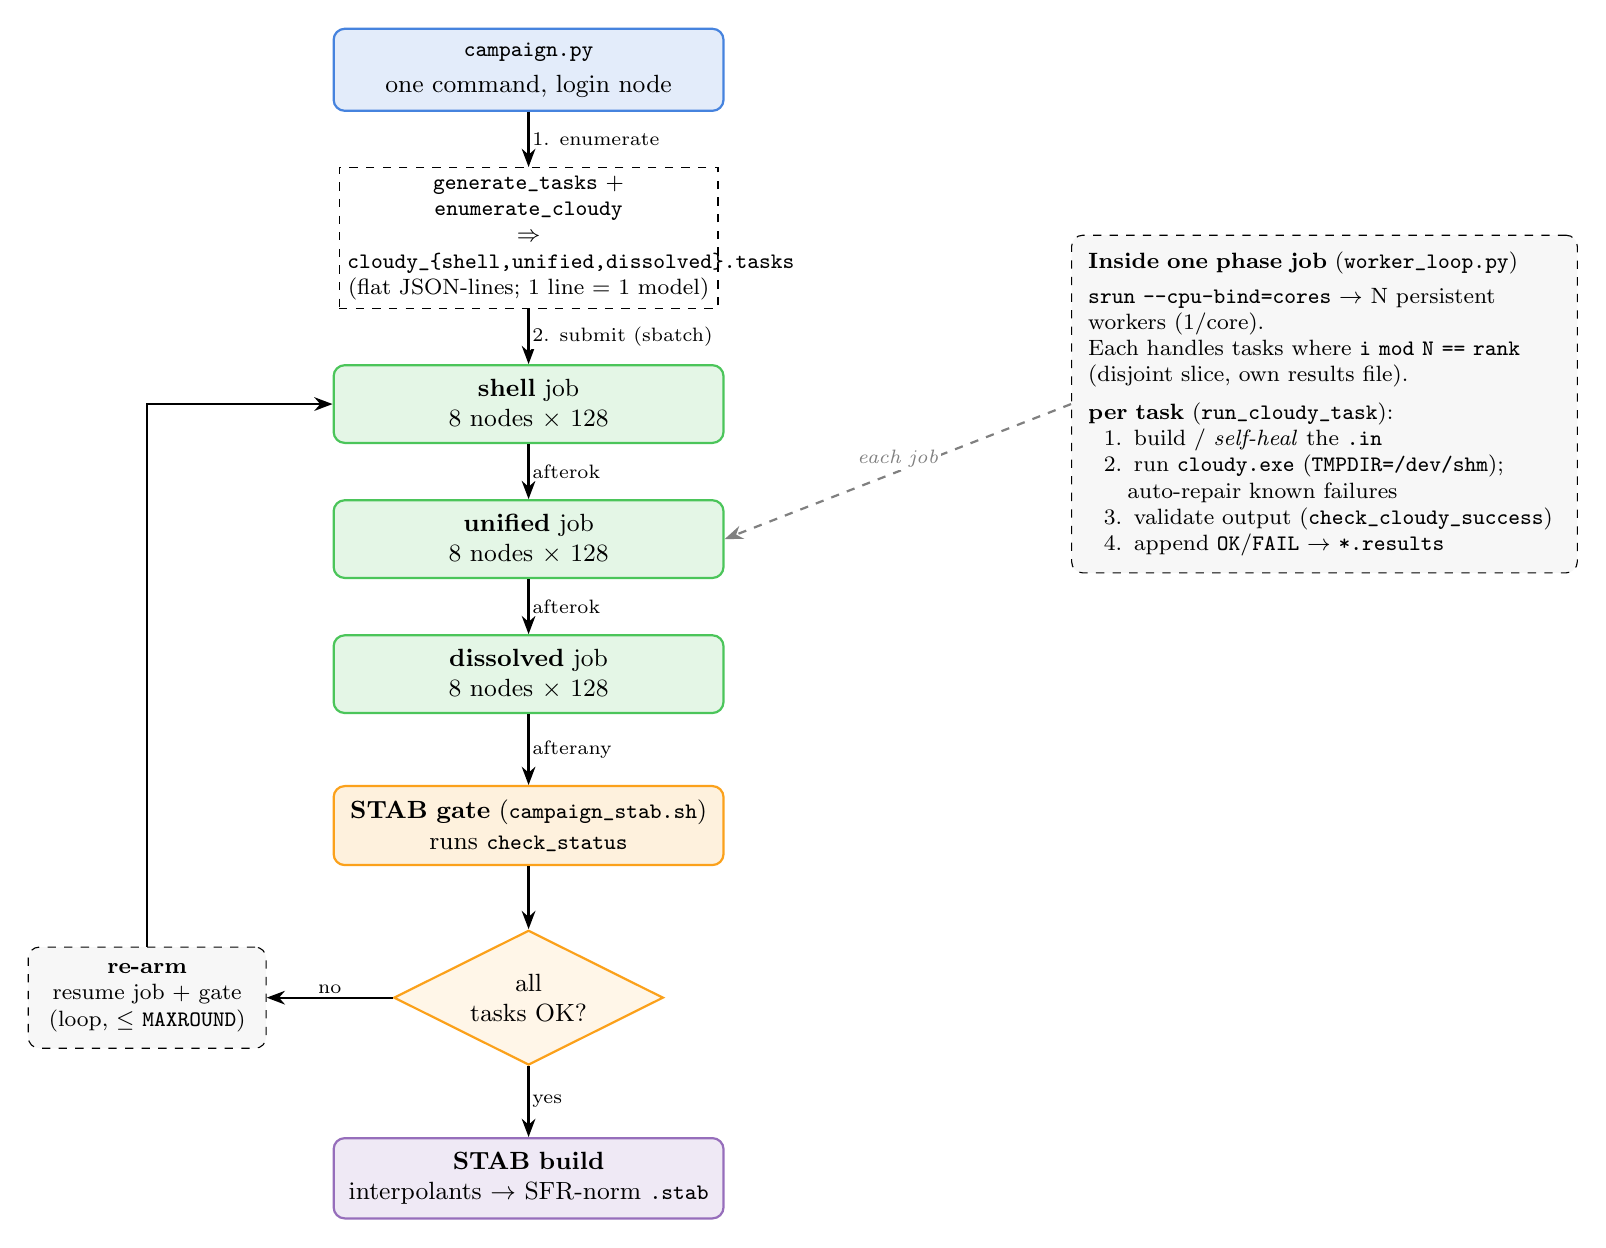
\begin{tikzpicture}[
  font=\small,
  >=Stealth,
  node distance = 7mm,
  pbox/.style   = {rectangle, rounded corners, draw, thick, align=center,
                   inner sep=5pt, text width=46mm},
  job/.style    = {pbox, fill=cJob!15, draw=cJob},
  login/.style  = {pbox, fill=cLogin!15, draw=cLogin},
  gate/.style   = {pbox, fill=cGate!15, draw=cGate},
  build/.style  = {pbox, fill=cBuild!15, draw=cBuild},
  dec/.style    = {diamond, aspect=2, draw, thick, align=center, inner sep=1pt,
                   fill=cGate!10, draw=cGate, text width=20mm},
  data/.style   = {rectangle, draw, dashed, align=center, font=\footnotesize,
                   inner sep=3pt, text width=46mm},
  detail/.style = {rectangle, rounded corners, draw, dashed, align=left,
                   font=\footnotesize, inner sep=6pt, text width=60mm, fill=black!3},
  arr/.style    = {->, thick},
  lab/.style    = {font=\scriptsize, fill=white, inner sep=1pt}]

% ---- left column: the orchestration chain ---------------------------------
\node[login] (camp) {\textbf{\code{campaign.py}}\\[2pt] one command, login node};
\node[data, below=of camp] (tasks)
   {\code{generate_tasks} + \code{enumerate_cloudy}\\
    $\Rightarrow$ \code{cloudy_{shell,unified,dissolved}.tasks}\\
    (flat JSON-lines; 1 line = 1 model)};
\node[job, below=of tasks] (shell)   {\textbf{shell} job\\ 8 nodes $\times$ 128};
\node[job, below=of shell] (unified) {\textbf{unified} job\\ 8 nodes $\times$ 128};
\node[job, below=of unified] (diss)  {\textbf{dissolved} job\\ 8 nodes $\times$ 128};
\node[gate, below=9mm of diss] (gate)
   {\textbf{STAB gate} (\code{campaign_stab.sh})\\ runs \code{check_status}};
\node[dec, below=8mm of gate] (dec) {all\\ tasks OK?};
\node[build, below=9mm of dec] (build)
   {\textbf{STAB build}\\ interpolants $\to$ SFR-norm \code{.stab}};

% chain arrows
\draw[arr] (camp) -- (tasks) node[lab, midway, right] {1. enumerate};
\draw[arr] (tasks) -- (shell) node[lab, midway, right] {2. submit (sbatch)};
\draw[arr] (shell) -- (unified) node[lab, midway, right] {afterok};
\draw[arr] (unified) -- (diss) node[lab, midway, right] {afterok};
\draw[arr] (diss) -- (gate) node[lab, midway, right] {afterany};
\draw[arr] (gate) -- (dec);
\draw[arr] (dec) -- node[lab, right] {yes} (build);

% ---- resume loop (no -> re-arm a fresh job + the gate, back to the top) ----
\node[detail, left=16mm of dec, text width=26mm, align=center] (resume)
  {\textbf{re-arm}\\ resume job + gate\\ (loop, $\le$ \code{MAXROUND})};
\draw[arr] (dec) -- node[lab, above] {no} (resume);
\draw[arr] (resume) |- (shell.west);

% ---- right: what one phase job actually does ------------------------------
\node[detail, right=44mm of shell, anchor=west] (worker)
  {\textbf{Inside one phase job} (\code{worker_loop.py})\\[3pt]
   \code{srun --cpu-bind=cores} $\to$ N persistent workers (1/core).\\
   Each handles tasks where \code{i mod N == rank} (disjoint
   slice, own results file).\\[4pt]
   \textbf{per task} (\code{run_cloudy_task}):\\
   \ \ 1. build / \emph{self-heal} the \code{.in}\\
   \ \ 2. run \code{cloudy.exe} (\code{TMPDIR=/dev/shm});\\
   \ \ \ \ \ auto-repair known failures\\
   \ \ 3. validate output (\code{check_cloudy_success})\\
   \ \ 4. append \code{OK}/\code{FAIL} $\to$ \code{*.results}};
\draw[arr, dashed, gray] (worker.west) -- (unified.east)
      node[lab, midway, above, font=\scriptsize\itshape] {each job};

% parallelism note (kept clear of the worker box, under the chain arrows)
\node[font=\scriptsize\itshape, align=center, below=1mm of diss, yshift=-0.5mm] {};

\end{tikzpicture}
\end{document}
